\subsection{WPT metoder}
De tre relevante metoder til trådløs energi, indebære induktiv magnetisk-, resonans magnetisk kobling og mikrobølger. Induktiv og resonans virker ved near-fields og mikrobølger virker ved far-ifelds.

\begin{figure}[H]
\centering
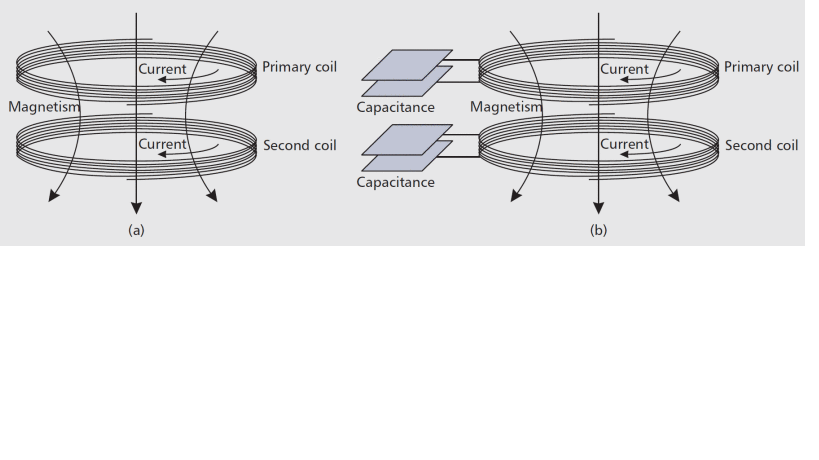
\includegraphics[scale=0.5]{Vildledning/Schematics/induktiv_resonans}
\caption{model af WPT setup}
\label{model af WPT setup}
\end{figure}

Induktiv kobling. 
WPT ved induktiv kobling fungere ved induktion over et magnetfelt mellem to spoler, hvilke genereres en strøm og spænding som ses på figure 2.4a. Magnetisk induktiv kobling sker, når den primærspole som fungere som energi senderen genererer et vekselene magnetfelt på tværs af den sekundærspole, der er energien modtageren. Dette sker inden for et området generelt mindre end bølgelængden. Denne process skaber en near-field kraft som induktiveres over den sekundære spole til en strøm/spænding, hvilke kan udnyttes af et trådløs apparatur, eksempelvis en mobil. 
Fordelen ved induktiv kobling inkludere følgende, teknologien er simple og nem at implementer ved høj effektivitet og det er sikkert for mennesker at være i nærheden. Den er dog begrænset af afstand fra transmitter og receiver, idet at den har en effektiv energioverførelse mellem nogle få millimeter til et par centimeter. Ulemper ved induktiv kobling indebære den relative korte ladeafstand, varmen der udvikles i spolerne og spolerne skal ligge meget tæt og så lige overfor hinanden som muligt for at opnå den optimale effekt.
Teknologien bliver i dag set i mobile enheder (mobiltelefoner og tablets), tandbørster, RFID-tags, induktionskomfur og betalingskort.

Resonans kobling. 
Magnetisk resonans kobling er baseret på kortvarige bølgekobling, hvilke genere og overføre en elektrisk strøm mellem to resonans spoler i et oscillerende eller varierende magnetfelt, som set på figure 2.4b. Da de to spoler er køre på samme resonans frekvens, kan der opnå en høj effektiv elektrisk energioverførelse, med meget lidt tab til  eksterne faktorer. Denne indskab gøre energioverførelsen næsten upåvirket af omgivelserne, hvilke også gør det muligt at lade selvom der er noget i mellem transmitter og receiver. 
Den klare fordel ved resonans kobling er den meget større effektive lade distance, som kan opnå en effekt på 90 procent optil 1 meter mellem transmitter og receiver, og 40 procent ud til to meter. Derudover kan en enkel transmitter lader flere receiver på samme tid så længe de operer på sammen resonans frekvens.
En ulemperne ved resonans kobling er at hver receiver kræver en dedikeret kapacitets spole, hvilke gøre det svært at gøre receiveren lille nok til mobile enheder, og det gøre det generelt mere kompliceret at implementer. 